\documentclass[english,11pt,twoside,a4paper]{article}
\usepackage[left=2cm,top=1cm,right=2cm,nohead,nofoot]{geometry}
\usepackage[utf8]{inputenc}
\usepackage{hyperref}
\usepackage{amssymb}
\usepackage{graphicx}
\usepackage{titling}
\newcommand{\subtitle}[1]{%
  \posttitle{%
    \par\end{center}
    \begin{center}\large#1\end{center}
    \vskip0.5em}%
}

\begin{document}
\author{
  Niemistö, Jesse
  \and
  Muona, Leo
  \and
  Hilden, Matias
}
\title{Raspberry Pi robot}
\subtitle{Intelligent Embedded Systems - Final report}

\maketitle

\tableofcontents

\section{Introduction}

This is a final report for the course Intelligent Embedded System (id 582711) at the CS Department of the University of Helsinki. This course was held at during Spring term 2014, third period. The course is a self-study course that consists of an embedded systems project. For our project we chose to build a Raspberry Pi robot, which utilizes Pi's camera module, audio output and electric DC motors.

Raspberry Pi is a cheap arm-computer that was originally created for the purpose to help more people to get into programming. We chose to use this one-chip-computer for our project because it runs on Linux (among other operating systems), it has a camera module available, it has GPIO pins for controlling a motor control chip, and all of our team members already had one lying around.

This document includes our project idea, requirements and initial design for the robot, implementation of the robot, evaluation of our project, and a summary of lessons learned. This is the tale of our awesome little raspi robot.

\section{The idea}

We got our initial idea from the video game Portal by Valve Corp. In the game, there were these "cute" robot turrets that recognized movement, talked to the source of the movement and shot them. So our initial idea was to create a robot similar to these turrets, so that we will use Raspberry Pi's camera module to recognize movement, target the movement source, and play a random audio clip to greet the source of the movement.

Our initial idea had two DC motors to control the turret's movement and a laser- or LED-pointer to point the target. However this idea evolved during the project just to use one motor and only turn the camera towards the movement source.

\section{Requirements and initial design}

At the start of our project we wrote our requirements and then initial design. The design consists more on actual planning of hardware part, than the code to be created. This section can be divided into five parts: required features, audio system design, camera design, motor control system design, and software design.

\subsection{Required features}

These were our required features at the start of our project when designing the robot:

\begin{itemize}
  \item Horizontal and vertical rotational movement.
  \item WAV (or ogg) audio playback.
  \item Motion detection based on frame difference algorithm.
  \item Aiming at detected movement.
  \item Remote control.
  \item Works on top of Linux.
\end{itemize}

We used these features a guideline for our project design. At this stage it is good to mention that some of these features were modified during the project.

\subsection{Audio design}

TODO

\subsection{Camera design}

We decided to use a simple plug-in Raspberry Pi camera module, which we will use to take pictures that we compare to previous ones to detect movement. Since Raspberry Pi has a ready-to-use socket for camera cable, no extra cables or power supplies are needed. To use the camera we will use \href{https://github.com/raspberrypi/userland}{Pi's Userland code}, that comes with raspistill-program which we can use to take still pictures.

\subsection{Motor control design}

To control the motors, we planned our design around L293D motor control chip, which is cheap and easily available. Our design consisted of two motors, one to turn the camera horizontally and one to turn the camera vertically. This design used two L293D chips, one for each motor.

\begin{figure}
  \begin{center}
    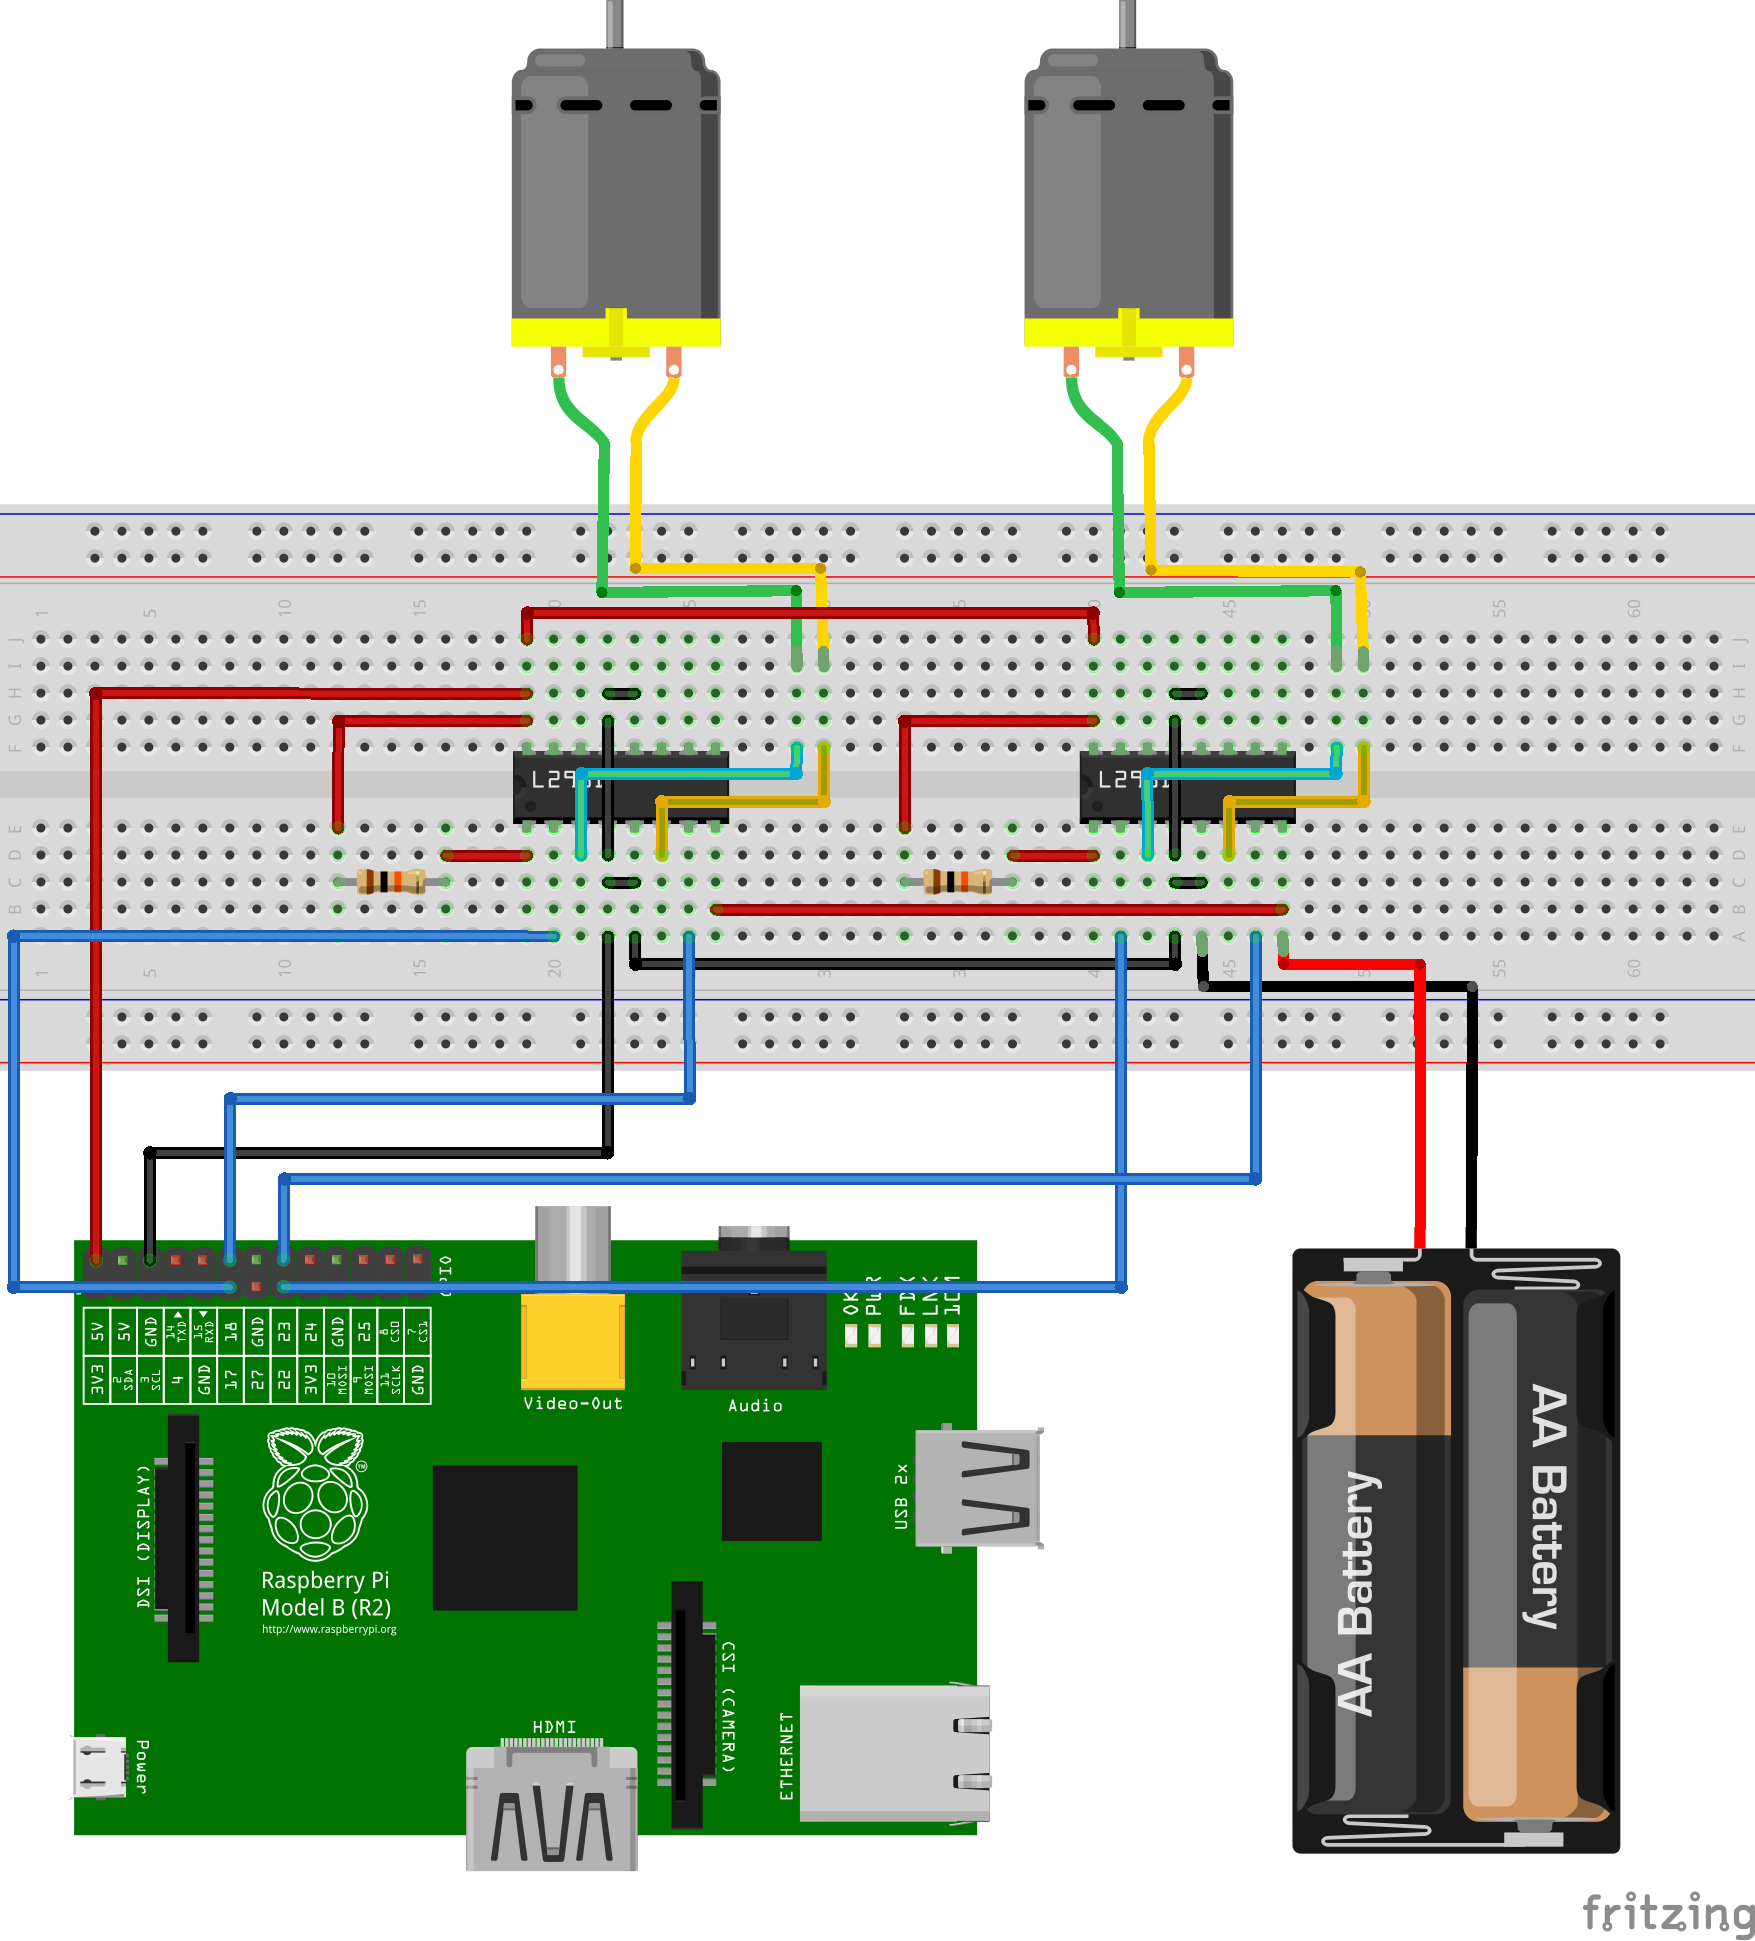
\includegraphics[scale=0.75]{motor_controllers_l293d_bb.png}
    \caption{Motor controllers design in breadboard view.}
  \end{center}
  \label{l293d_bb_design}
\end{figure}

Figure \ref{l293d_bb_design} shows how the chips would be connected into the Raspberry Pi. Design uses GPIO pins 17 and 18 to control the first motor and pins 22 and 23 to control the second motor. The two AA batteries will supply power for both of the motors, and Raspberry Pi will supply power for the motor control chips.

\subsection{Software design}

Our project requires software for three main things: camera control, audio control and motor control. Even though we use a ready-to-use software to take pictures with the camera, we need to write our own software for image analysis, that is used to detect movement in the camera. We will write our own audio playback code against pulseaudio sound server. As for sound files, we are planning to use .ogg files. For the motor controlling we plan to use either direct /dev/mem code, or an additional \href{http://wiringpi.com}{WiringPi gpio library} to control the GPIO pins.

We will also write other code, like the logical code for the whole software, threading for different parts, and a remote control code for testing purposes. And hopefully we don't need to write multiple hacks.

\section{Implementation}

For the implementation, we ran into few problems along the way. Implementation was divided into three separate parts: motor related stuff, audio related stuff and camera related stuff. These parts were implemented as paraller. During the implementation, few features needed some modification and later of the project timetable few "nasty" code and hacks were implemented to get the wanted results.

\subsection{Motor control system}

Largest modifications to the design had to be done to the motor controlling system. After implementing the planned two-motor-system, we noticed that it would be hard to create correct platform that would be aimed in two dimensions. In addition to this, we noticed that we couldn't implement the correct calculations for vertical movement during project's timetable. Thus we changed the motor system to use only horizontal motor.

\begin{figure}
  \begin{center}
    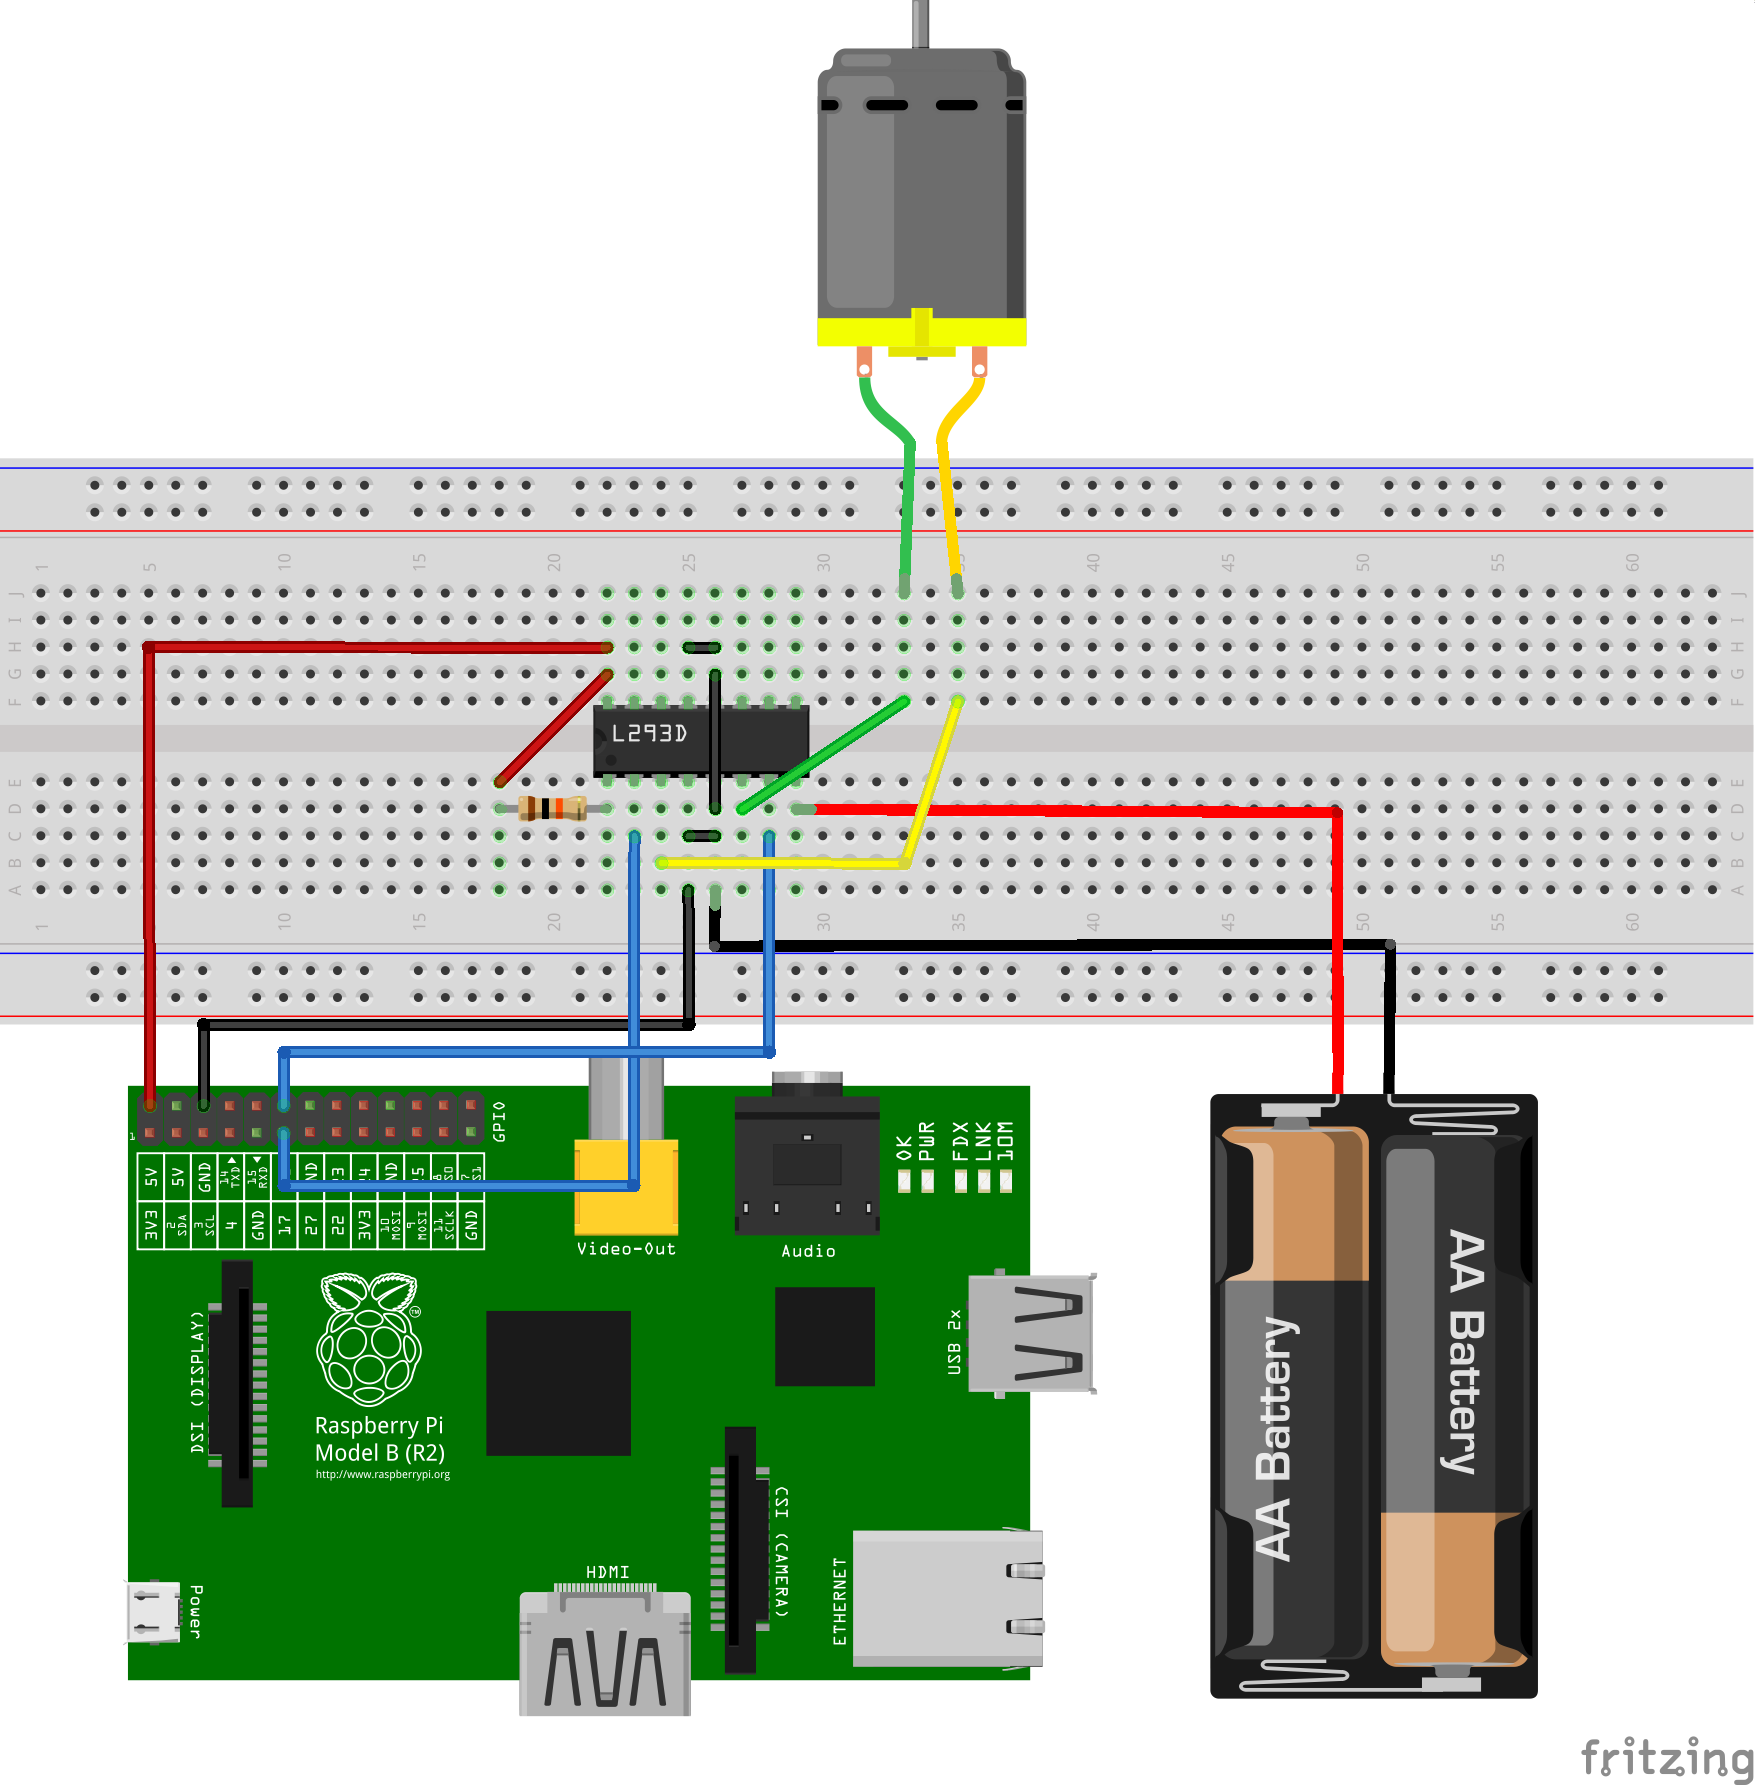
\includegraphics[scale=0.75]{motor_controllers_l293d_impl_bb.png}
    \caption{Motor controller implementation in breadboard view.}
  \end{center}
  \label{l293d_bb_impl}
\end{figure}

The hardware implementation of our motor system is shown in figure \ref{l293d_bb_impl}. The AA batteries now have to supply only one motor, and we had to implement code for only two GPIO pins. The L293D motor control chip we used gets it's VCC1 power from Raspberry Pi's 5V pin, and uses that same line trought a 10k ohm resistor to give the enable signal for our motor chip.

Motor control's software had some changes as well. After we started to use \href{http://wiringpi.com}{WiringPi library} the software had to be run as root, as it was WiringPi's requirement. This caused us some problems with pulseaudio, which has a lot of problems when run as root. A fix to this was to remove WiringPi linking from our software and add WiringPi library only as a system requirement. That is, it should be installed on the Raspberry Pi normally. Then we used system calls to use gpio-program, that was bundled with WiringPi and could be run in non-root environments. This is one of the hacks we had to do to get things working.

\section{Evaluation}

Motor controlling system worked well. Mainly due to the hack we made and the fact that the L293D chip is a pretty simple control chip. Using the GPIO pins is pretty straight forward with the WiringPi library. Only bad thing in the motor control system implementation is that we had to downgrade our project to use only one motor instead of two.

\section{Summary}

TODO

\end{document}
